\newpage
\section{(R) Space Discretization - Avoidance Grid}\label{s:AvoidanceGrid}

\paragraph{Operation Space:} The \emph{Operation Space} is a space where UAS can effectively surveillance its surroundings.

The\emph{Discrete Situation Evaluation} is bounded to\emph{UAS} specific\emph{position} and\emph{orientation} in fixed\emph{time} $t_i$. To enable\emph{deterministic evaluation} the\emph{operation space} needs to be segmented into\emph{finite set} of space portions. The\emph{finite operation space segmentation} is usually done by\emph{Grid} segmentation, which distributes space into portions with solid boundary.

The \emph{Main Sensor} is \emph{LiDAR} (problems \ref{eq:basicProblemDefinition}.-\ref{pro:rulesOfTheAir}.). The \emph{effective occupancy computation} \cite{homm2010efficient} is given by clustering \emph{LiDAR} field of vision into \emph{polar coordinates grid}.

The \emph{point} scanned by \emph{LiDAR}, where \emph{UAS position} is center of \emph{local coordinate frame} and \emph{UAS heading is defining the main axes} is given as:

\begin{equation*}
    point = [distance,horizontal^\circ,vertical^\circ].
\end{equation*}

\begin{note}
    For polar/euclidean transformations and local/global coordinate frames refer to background theory (sec. \ref{sec:complementsOfAlgebra}). 
    
    The \emph{right side} of UAS $horizontal^\circ$ $]-\pi,0[$, the \emph{left side} of UAS $horizontal^\circ$ $\in$ $[0,\pi]$, the \emph{down side} of UAS $vertical^\circ$ $]-\pi,0[$, the \emph{top side} of UAS $vertical^\circ$ $\in$ $[0,\pi]$
\end{note}

\paragraph{LiDAR Reading Space Segmentation:} The \emph{polar space} can be separated into cells, which bounds the portion the space, similar to \emph{euclidean} space grid. The \emph{reason} for this segmentation is \emph{LiDAR} reading density\footnote{Example rotary LiDAR Velodyne VL-16 specs: \url{https://www.cadden.fr/wp-content/uploads/2017/02/Velodyne_VLP-16-Puck.pdf}}. The \emph{polar space portions} state can be assessed directly, the \emph{polar $\to$ euclidean} coordinate frame transformation is not time-effective. The \emph{polar space} assessment of \emph{Lidar Data} has minimal complexity and it is cost effective. \cite{gupta2010comparative}.

\begin{definition}{Space partition - cell}\label{def:cell}
    The \emph{cell} is a portion of space in UAS local polar coordinate frame, given by:
    \begin{enumerate}
        \item \emph{Distance Range} -  bounded by $distance_{start}$ $<$ $distance_{end}$ $in$ $\R^+$.
        \item \emph{Horizontal Range} - bounded by $horizontal^\circ_{start}$ $<$ $horizontal^\circ_{start}$ $\in$ $]-\pi,\pi]$.
        \item \emph{Vertical Range} - bounded by $vertical^\circ_{start}$ $<$ $vertical^\circ_{start}$ $\in$ $]-\pi,\pi]$.
    \end{enumerate}
    
    \noindent The \emph{bounded space} for \emph{cell} is defined as:
    
    \begin{multline}\label{eq:boundedSpaceCell}
        Bounded Space(cell)=\dots\\
            \left \{
                \begin{aligned}
                point& \in \R^3 \text{ where}:\\
                    &\left(\begin{aligned}
                        cell.distance_{start} &<& point.distance &\le& cell.distance_{end},\\
                        cell.horizontal^\circ_{start} &<& point.horizontal^\circ &\le&  cell.horizontal^\circ_{end},\\
                        cell.vertical^\circ_{start} &<& point.vertical^\circ &\le& cell.vertical^\circ_{end}\\
                    \end{aligned}\right)
                \end{aligned}
            \right\}
    \end{multline}
    
    \noindent For one \emph{LiDAR Scan} the \emph{hits set} is given as \emph{set} of \emph{all points} which lands in bounded cell space:
    \begin{equation}\label{eq:LidarHitsCell}
        Lidar Hits (cell) = \left\{point \in Lidar Scan:  point \in Bounded Space(cell)\right\}    
    \end{equation}
    
    The \emph{passing hits} for cell are hits which are going trough the cell (passing), but it lands in distance greater than $cell.distance_{end}$, defined as:
    \begin{multline}\label{eq:passingHitsCell}
        Passing Hits(cell)=
        \dots\\
            \left \{
                \begin{aligned}
                point& \in Lidar Scan \text{ where}:\\
                    &\left(\begin{aligned}
                        cell.distance_{end}&<& point.distance &&,\\
                        cell.horizontal^\circ_{start} &<& point.horizontal^\circ &\le&  cell.horizontal^\circ_{end},\\
                        cell.vertical^\circ_{start} &<& point.vertical^\circ &\le& cell.vertical^\circ_{end}\\
                    \end{aligned}\right)
                \end{aligned}
            \right\}
    \end{multline}
\end{definition}

\begin{note}
    The \emph{cells} with same \emph{distance} range form \emph{layers}. The \emph{greater} the distance from \emph{coordinate frame} origin the \emph{greater} volume of the cell.     
\end{note}

\paragraph{Effective Operation Space - Avoidance Grid:} Let start with example, the UAS  (fig. \ref{fig:LidarSpaceSegmentation}). 

\begin{figure}[H]
    \centering
    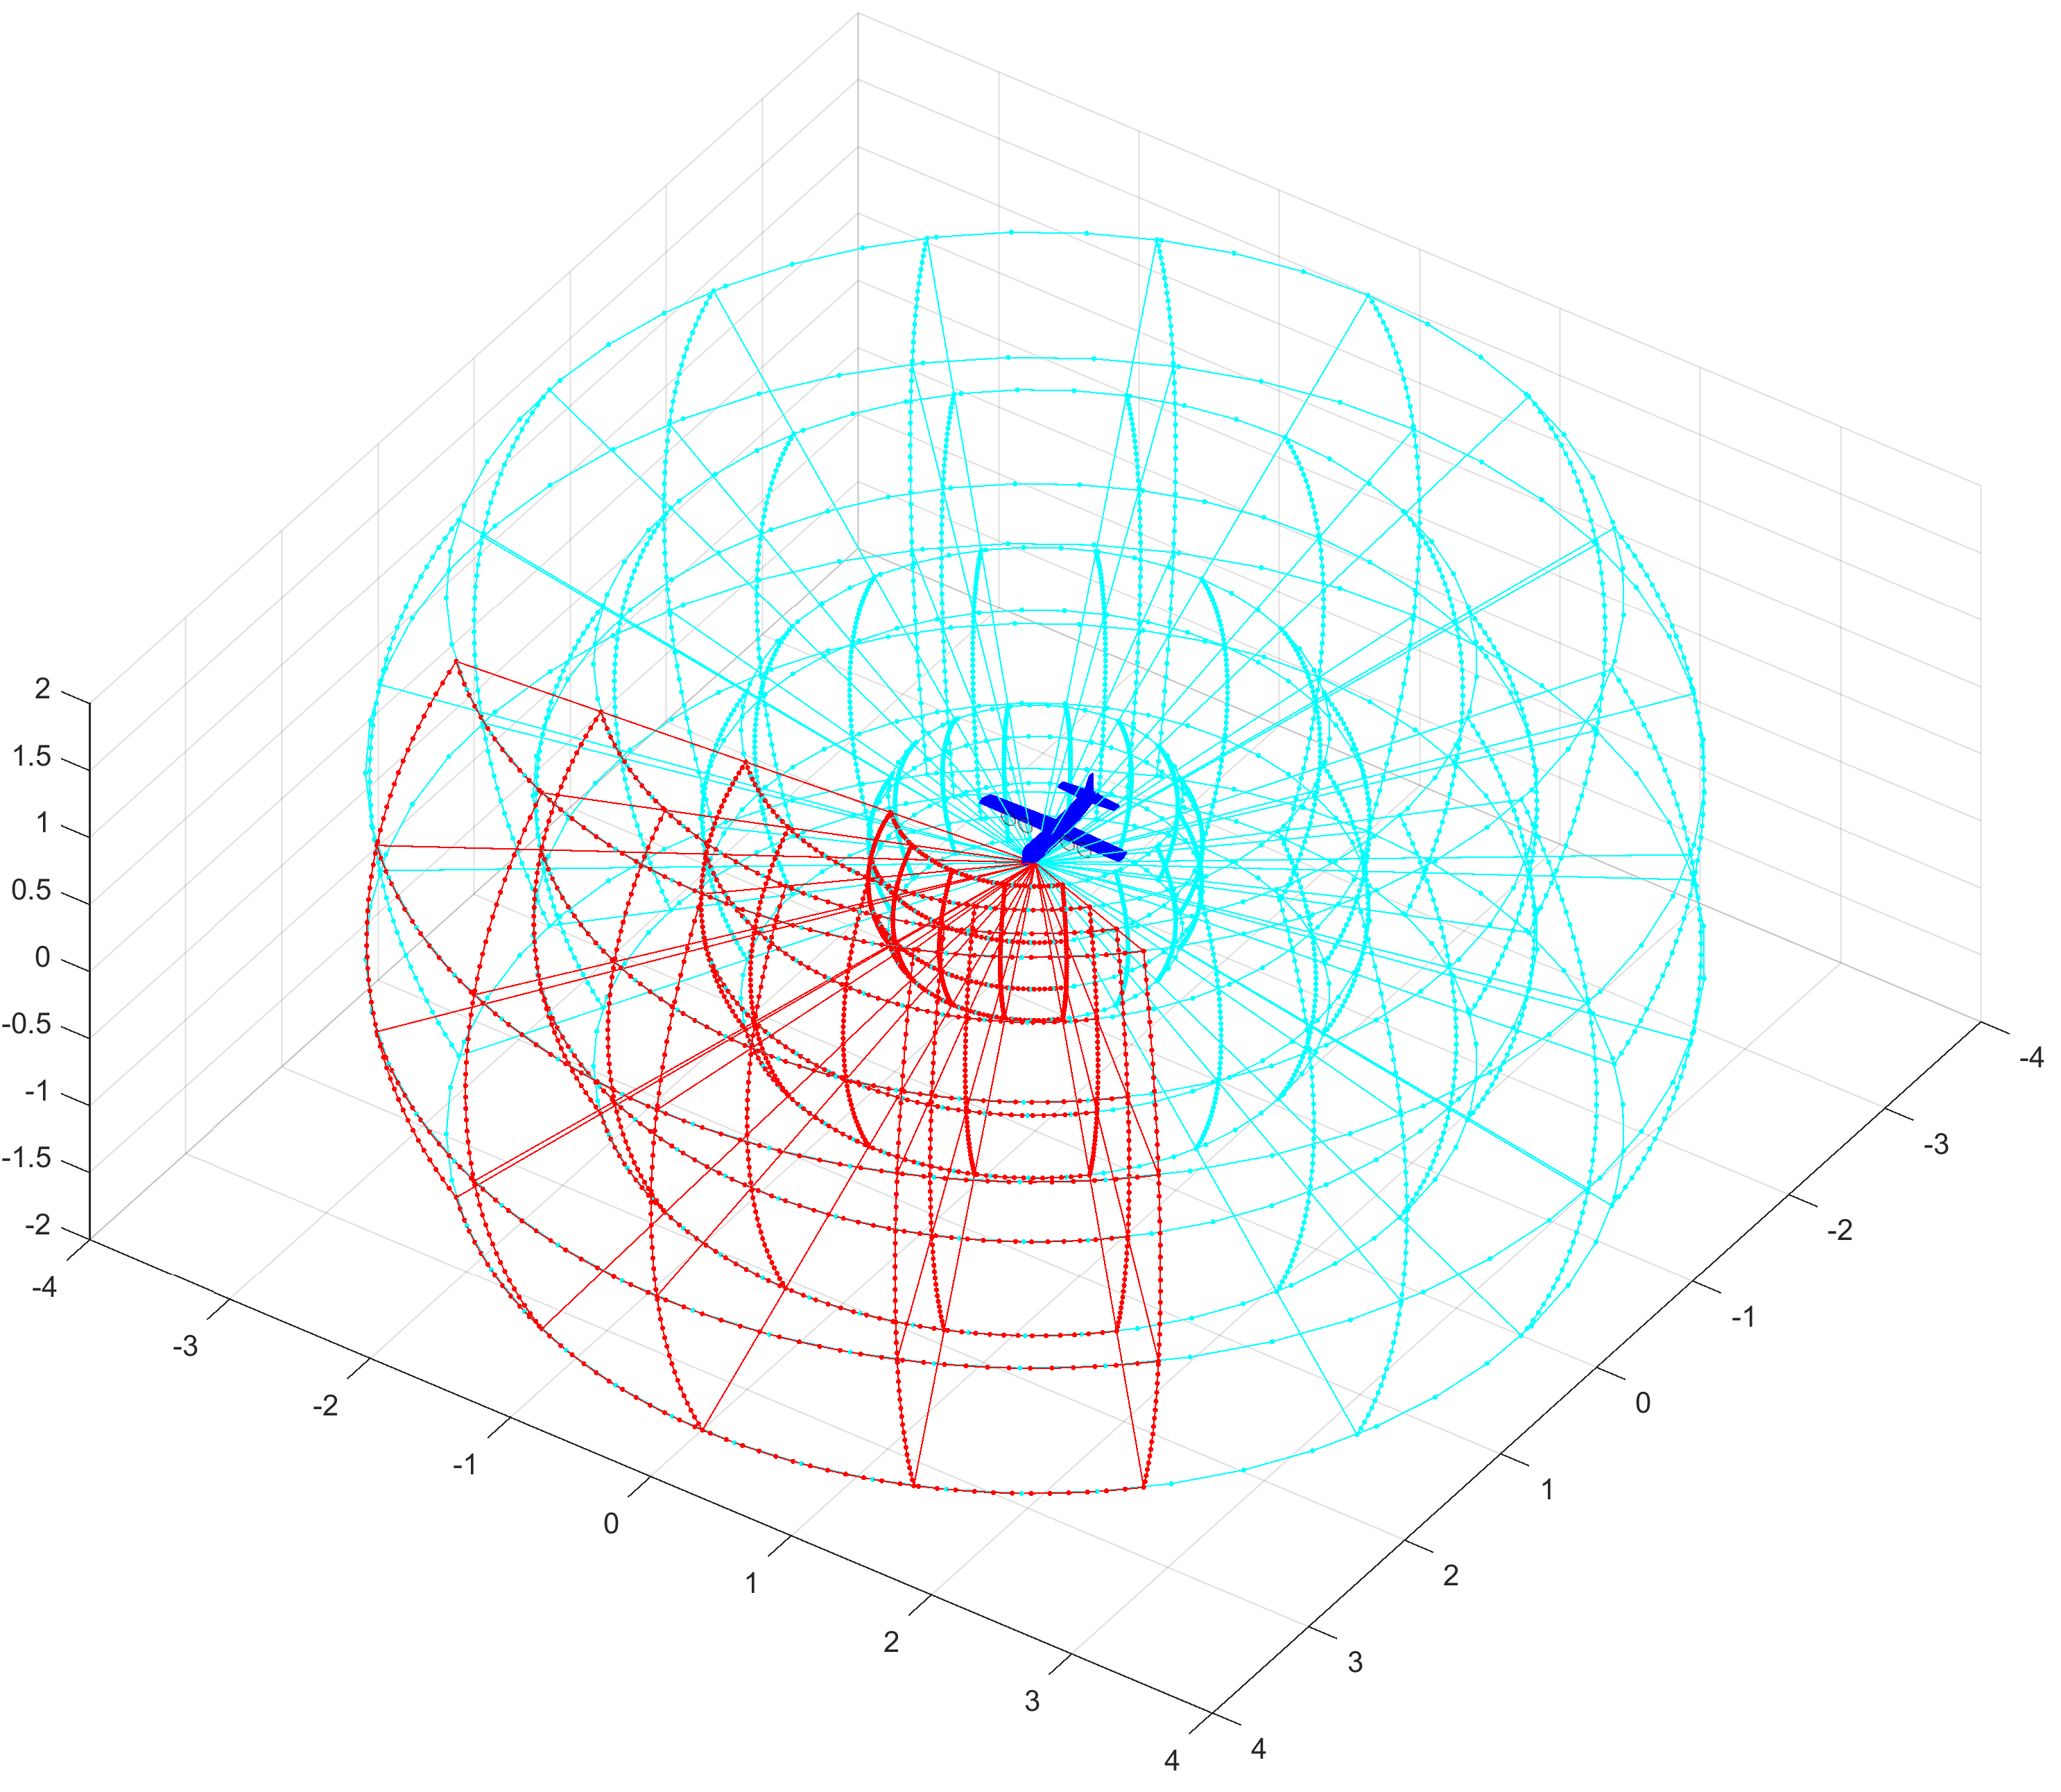
\includegraphics[width=0.80\linewidth]{\FIGDIR/TE046LiDARRasterRange} 
    \caption{Example: The \emph{LiDAR} reading segmentation - cells.}
    \label{fig:LidarSpaceSegmentation}
\end{figure}

The \emph{full LiDAR Swipe} (cyan and red lines) of \emph{UAS} (blue plane) has \emph{shape} of conical cylinder. Under \emph{ideal circumstances} the \emph{LiDAR swipe} would have \emph{ball shape}, but in real cases the \emph{craft body portion} where \emph{LiDAR} is mounted is unused.

\newpage
The \emph{frontal portion} (red line) is a set of cells where \emph{UAS} can make maneuver. The \emph{red portion} size is determined by \cite{zaiane2002clustering}:

\begin{enumerate}
        \item \emph{Sensors ranges} - the union of \emph{effective sensor ranges} defines the maximal \emph{effective space boundary}, because there is no reason to asses situation over effective \emph{sensor range}.
        
        \item \emph{Information sources} impact - there is no real impact on \emph{effective space boundary}.
        
        \item \emph{UAS maneuverability} - the \emph{Reach Set} (sec. \ref{s:ReachSets}) gives optimal \emph{effective space boundary}, because there is no need to assess the situation out of \emph{reachable space} or its vicinity. 
        
        \item Computation power - the \emph{Reach Set Evaluation} and \emph{Intersection} algorithms are \emph{scaling} with \emph{effective space boundary}.
        
        \item Airworthiness requirements - the \emph{regulations} can impose some minimal requirements on \emph{effective space boundary}.
\end{enumerate}


\begin{definition}{Avoidance Grid}\label{def:AvoidanceGrid} The \emph{effective space boundary} (fig. \ref{fig:LidarSpaceSegmentation} red lines) given by a portion of space in UAS local polar coordinate frame, bounded by:
    \begin{enumerate}
        \item \emph{Distance Range} -  bounded by $distance_{start}$ $<$ $distance_{end}$ $in$ $\R^+$.
        \item \emph{Horizontal Range} - bounded by $horizontal^\circ_{start}$ $<$ $horizontal^\circ_{start}$ $\in$ $]-\pi,\pi]$.
        \item \emph{Vertical Range} - bounded by $vertical^\circ_{start}$ $<$ $vertical^\circ_{start}$ $\in$ $]-\pi,\pi]$.
    \end{enumerate}

\noindent Separated into \emph{layers} depending on the distance and \emph{layer count}:
\begin{equation}\label{eq:avoidanceGridCellDistanceRange}
    \begin{aligned}
        layer^i_{start} & = (i-1)\times\frac{distance_{end}-distance_{start}}{layer Count}\\
        layer^i_{end} & = i\times\frac{distance_{end}-distance_{start}}{layer Count}
    \end{aligned};\quad i\in 1\dots I
\end{equation}

\noindent Layer horizontal/vertical separations separations defined by horizontal/vertically cell count:

\begin{equation}\label{eq:avoidanceGridCellHorizontalRange}
    \begin{aligned}
        horizontal^j_{start} & = (j-1)\times\frac{horizontal^\circ_{end}-horizontal^\circ_{start}}{horizontal Count}\\
        horizontal^j_{end} & = j\times\frac{horizontal^\circ_{end}-horizontal^\circ_{start}}{horizontal Count}
    \end{aligned};\quad j\in 1\dots J
\end{equation}

\begin{equation}\label{eq:avoidanceGridCellVerticalRange}
    \begin{aligned}
        vertical^k_{start} & = (k-1)\times\frac{vertical^\circ_{end}-vertical^\circ_{start}}{vertical Count}\\
        vertical^k_{end} & = k\times\frac{vertical^\circ_{end}-vertical^\circ_{start}}{vertical Count}
    \end{aligned};\quad k\in 1\dots K
\end{equation}

\noindent Then $cell_{i,j,k}$ given by (def. \ref{def:cell}) is member cell of Avoidance Grid for boundaries:
\begin{enumerate}
    \item \emph{Cell Distance Range} (eq. \ref{eq:avoidanceGridCellDistanceRange}) depending on layer index $i$.
    
    \item \emph{Cell Horizontal Range} (eq. \ref{eq:avoidanceGridCellHorizontalRange}) depending on horizontal index $j$.
    
    \item \emph{Cell Vertical Range} (eq. \ref{eq:avoidanceGridCellVerticalRange}) depending on horizontal index $k$.
\end{enumerate}

\noindent The example of \emph{Avoidance Grid Cells} is given in (fig. \ref{fig:LidarSpaceSegmentation} red boundary). 

The \emph{Avoidance Grid} is then given as set of cells:

\begin{equation}\label{eq:avoidanceGridCellSpace}
    Avoidance Grid = \bigcup cell_{i,j,k} \forall i \in 1\dots I, j\in 1\dots J, k\in 1\dots K
\end{equation}
\end{definition}

\paragraph{Trajectory Intersection:} The \emph{trajectory} intersection with \emph{Avoidance Grid} is solved in context of \emph{Reach Set Approximation} (def. \ref{def:ContainedReducedReachSet}). 
\begin{note}
    The \emph{trajectory intersection} function does not have an impact on \emph{Reach Set Approximation}, because its done prior the flight.
\end{note}


\paragraph{Grid Scaling:} For \emph{Sensor Field} there is \emph{effective sensor boundary} given as set:
\begin{equation}
    Boundary(Sensor \in Sensor Field) = \{points \in \R^3: \text{where reliable}\}
\end{equation}

\noindent The \emph{Boundary} for sensor fields is then given as \emph{union of all singe sensor boundaries}:

\begin{equation}
     Boundary(Sensor Field) = \bigcap_{\forall Sensors} Boundary(Sensor \in Sensor Field)
\end{equation}

\noindent Depending on boundary properties it can be projected into maximal avoidance grid boundary values:
\begin{equation}
    Boundary(Sensor Field) \to Avoidance Grid : 
    \begin{gathered}
        \max(distanceRange)\\
        \max(horizontalRange)\\
        \max(verticalRange)\\
    \end{gathered}
\end{equation}

\noindent Our approach taken worst LiDAR performance into account \cite{sabatini2014lidar} and following parameters for avoidance grid were calculated:

\begin{enumerate}
    \item distance range $[0m,10m]$,
    \item horizontal range $]-180^\circ,180^\circ]$,
    \item vertical range $[-30^\circ,30^\circ]$.
\end{enumerate}

\noindent The \emph{count of layers} is derived from \emph{average distance traveled by one movement application}:

\begin{equation}
    layer Count = \frac{|distance Range|}{\text{avg.}\quad length(movement\in Movement Set)}
\end{equation}

\noindent The \emph{layer length} is based on \emph{our movement set} (tab. \ref{tab:movements1}, \ref{tab:movements2}) the average movement length is 1 m, therefore the \emph{layer count} is 10.

The \emph{efficient boundary} is given by  \emph{Reach Set}. Estimate reach set coverage space using \emph{ellipsoidal toolbox} \cite{kurzhanskiy2006ellipsoidal} up to given \emph{sensor field} maximal distance:

\begin{equation}
    Boundary(Reach Set) = Ellipsoid(UAS System,distance)
\end{equation}

\noindent The values for \emph{Reach Set Boundary} with distance 10 m was following:
\begin{enumerate}
    \item distance range $[0m,10m]$,
    \item horizontal range $[-45^\circ,45^\circ]$,
    \item vertical range $[-45^\circ,45^\circ]$,
\end{enumerate}

\noindent The \emph{Avoidance Grid} boundary is given as \emph{intersection} of all boundaries:

\begin{equation}
    Boundary(Avoidance Grid) =  Boundary(Reach Set) \cap Boundary(Sensor Field)
\end{equation}

\noindent The values for \emph{Avoidance Grid Boundary} for our UAS system (sec. \ref{s:UASNonlinearModel}) following:
\begin{enumerate}
    \item distance range $[0m,10m]$,
    \item horizontal range $[-45^\circ,45^\circ]$,
    \item vertical range $[-45^\circ,45^\circ]$,
    \item layer count $10$, layer distance 1m.
\end{enumerate}

The \emph{horizontal cell count} and \emph{vertical cell count} was estimated by \emph{rule of thumb} to have value 7 and 5.

\paragraph{Cell in Avoidance Grid Properties:}\noindent For each cell $\vec{p}\in\R^3$ in the there are properties to be checked:

\begin{enumerate}
    \item \emph{Is there visibility to the cell ?} - how good is an observation of the cell by Sensor Field.
    
    \item \emph{Is there threat present ?} - how sure the data fusion is that there is eminent threat in the cell.
    
    \item \emph{Is the cell reachable ?} - if there is any trajectory which can get UAS to that cell without too much threat along the way.
\end{enumerate}

\noindent The answers to these questions will be given later (tab. \ref{tab:defuzificationRatings}).
